\section{Comparing implementation and diagonalization}

We also want to test our RBM implementation's computation time against the standard diagonalization algorithms. It is expected that the RBM only stands a chance to overtake these algorithms at large matrix sizes. For the Lipkin model we have used the symmetry of the total spin to to essentially reduce the size of the Hamiltonian. On the other hand the Pairing model Hamiltonian matrix could also be reduced by the fact that large parts of it is only zeros. Because of this we will look at the case of the Ising and Heisenberg models, but with the Ising model Hamiltonian only as the size evolves by $2^N\times 2^N$ for both cases. With the Ising model using $100 000$ Monte Carlo cycles each epoch of the learning process, with $500$ epochs in total, we get the following:

\begin{figure}[H]
  \begin{center}
    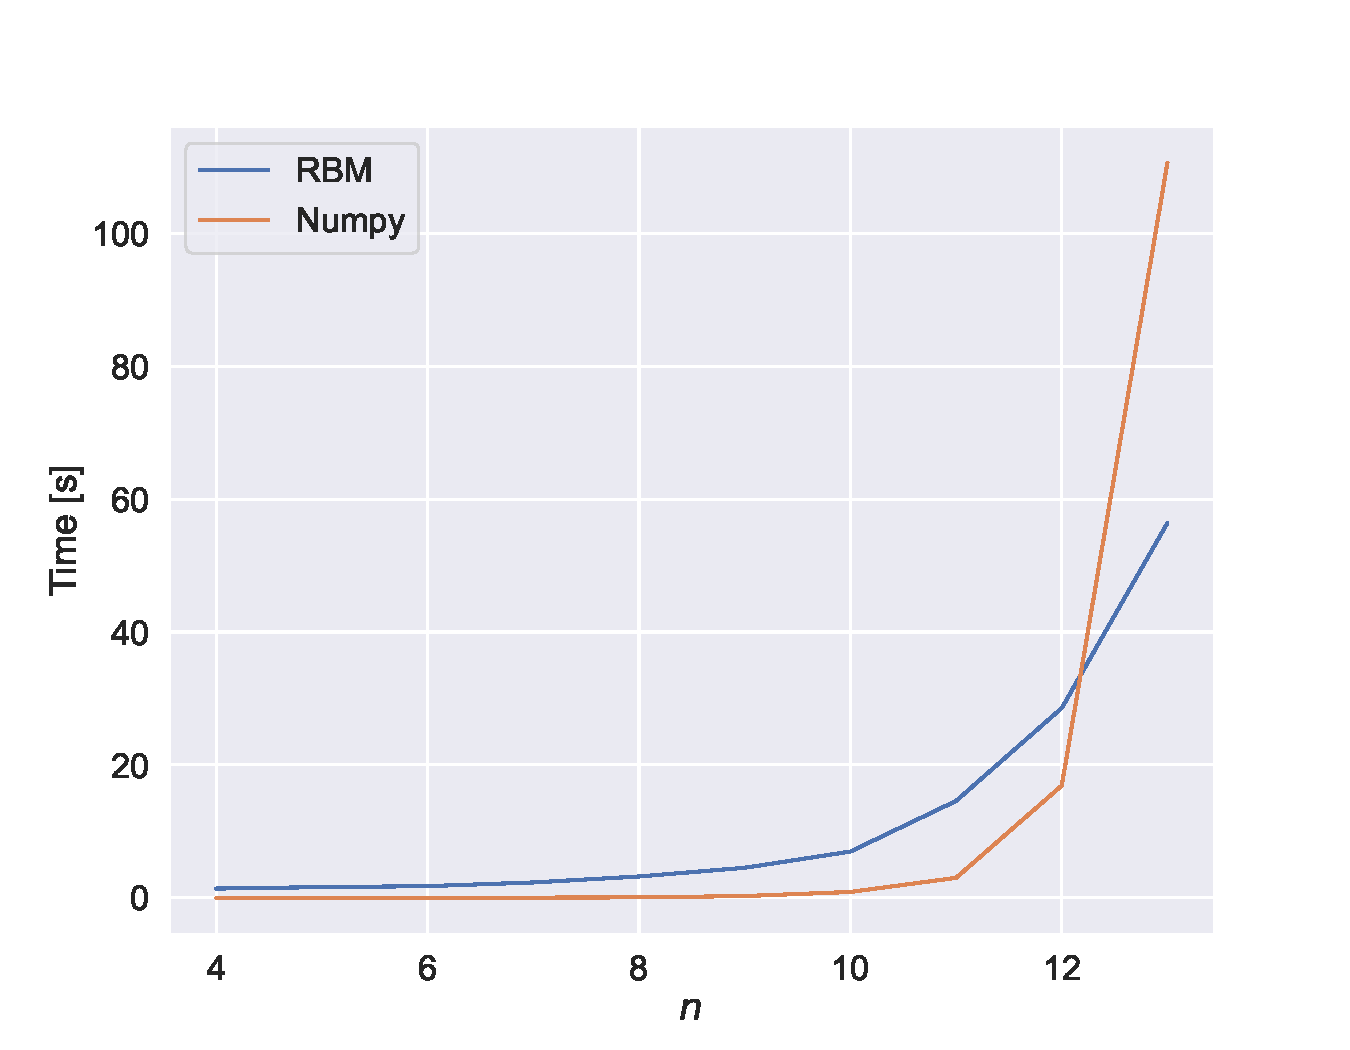
\includegraphics[width=0.95\textwidth]{Figures/Plots/Ising/[particles][4-13][e=500][J=0.3][L=-0.4]}
  \end{center}
  \caption{The computation time for finding the ground state energy for the Ising model with our implemented RBM compared with the time used by traditional diagonalization algorithms. Each data point is averaged over twenty runs. The diagonalization method used is \mintinline{python}{numpy.linalg.eigvals}.}
\end{figure}

We see that for the lower particle counts the standard diagonalization technique is superior, but as the Hamiltonian matrix size increases the RBM overtakes it at our last data point $n=13$. Here we use a algorithm that is for diagonalizing a general square matrix, but a more efficient version could be used, \mintinline{python}{numpy.linalg.eigvalsh}, as we are really dealing with sparse matrices. Comparing the RBM with the more efficient diagonalization algorithm we get:

\begin{figure}[H]
  \begin{center}
    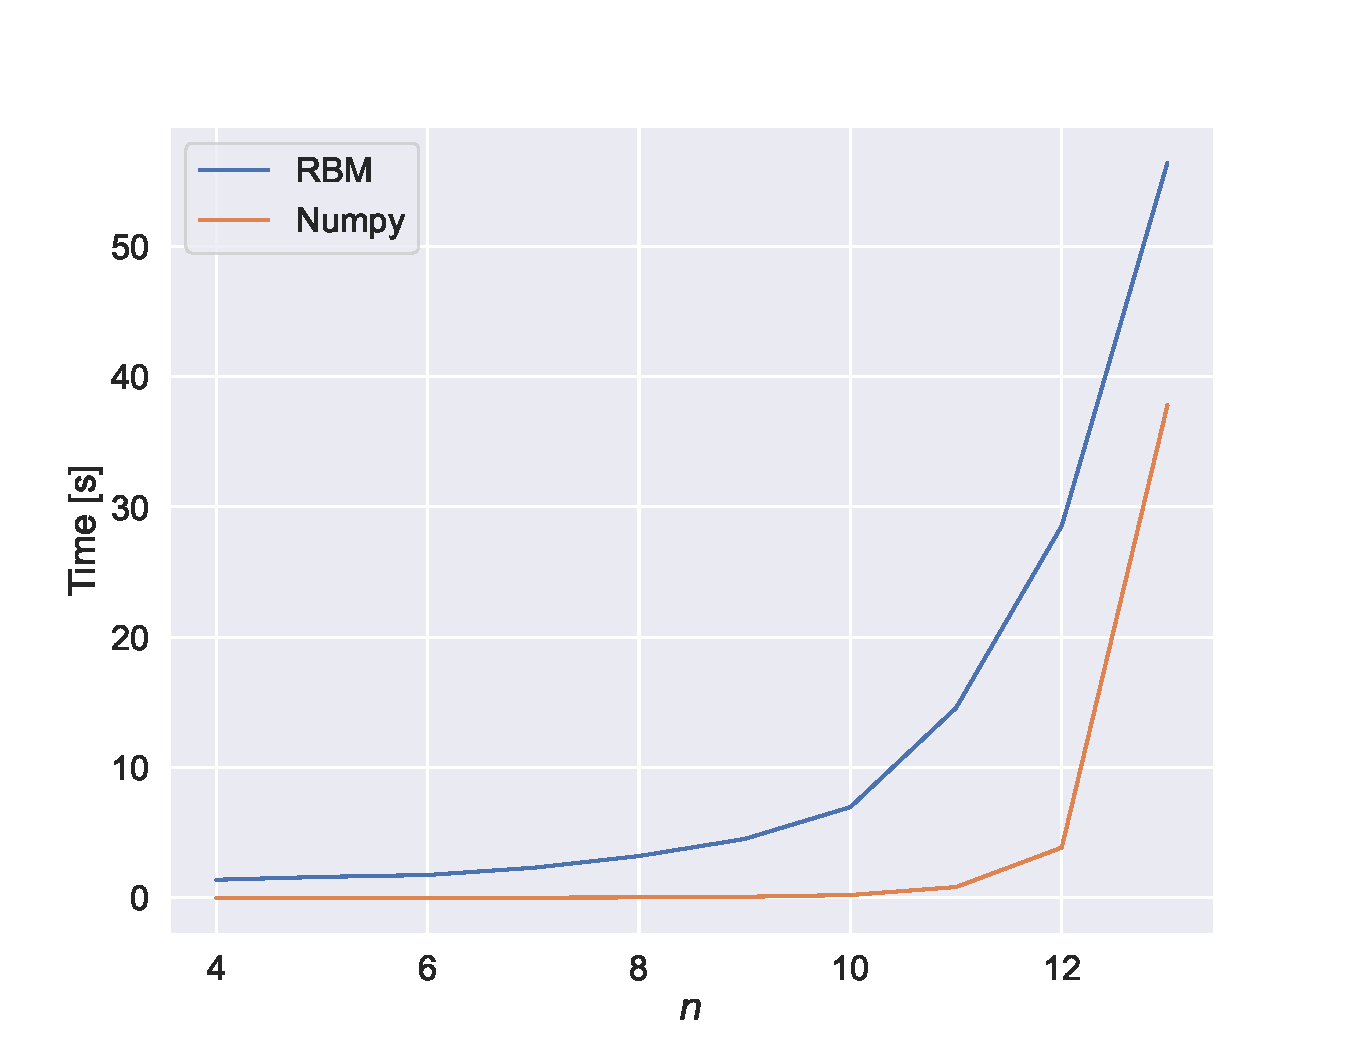
\includegraphics[width=0.95\textwidth]{Figures/Plots/Ising/[particles][4-13][e=500][J=0.3][L=-0.4][eigvalsh]}
  \end{center}
  \caption{The computation time for finding the ground state energy for the Ising model with our implemented RBM compared with the time used by traditional diagonalization algorithms. Each data point is averaged over twenty runs. The diagonalization method used is \mintinline{python}{numpy.linalg.eigvalsh}.}
\end{figure}

And we see that the RBM has once again fallen behind. It does seem like the \mintinline{python}{eigvalsh} algorithm still has a steeper incline at the $n=13$ mark, so one can assume here the RBM implementation would overtake it at even greater system sizes.



